\documentclass{article}

% Language setting
% Replace `english' with e.g. `spanish' to change the document language
\usepackage[polish]{babel}

% Set page size and margins
% Replace `letterpaper' with `a4paper' for UK/EU standard size
\usepackage[a4paper,top=2cm,bottom=2cm,left=3cm,right=3cm,marginparwidth=1.75cm]{geometry}

% Useful packages
\usepackage{amsmath}
\usepackage{graphicx}
\usepackage{listings}
\usepackage[pdftex,
            pdfauthor={Michał Czyż, Dawid Głąb},
            pdftitle={PK4 - Opis Projektu},
            pdfsubject={Opis Projektu},
            pdfkeywords={PK4, Projekt, Opis},
            pdfproducer={Latex with hyperref},
            pdfcreator={pdflatex},
            colorlinks=true,
            allcolors=blue]{hyperref}
\usepackage[T1]{fontenc}

\title{Projekt PK4: Platforma NLP}
\author{Dawid Głąb}

\begin{document}
\maketitle

\section{Wstęp}

Projekt do wykonania w tym semestrze to platforma nlp. Jest to akronim od przetwarzania języka naturalnego \textit{(eng. natural langugage processing)}. W ramach projektu zaimplementowane zostanie tłumaczenie tekstu z jednego języka na drugi oraz badanie sentymentu, czyli ocena tekstu pod względem użytego słownictwa

\section{Opis projektu}

Projekt będzie się składał z trzech głównych części:

\begin{itemize}
  \item Core - napisany w C++, główna część programu analizująca sentyment i tłumacząca tekst.
  \item Middleware - serwer API, łączący komunikację między programem, a interfejsem sieciowym.
  \item Frontend - strona internetowa korzystająca z API aby komunikować się z programem, główna część odpowiedzialna za komunikację użytkownika z programem.
\end{itemize}

Założenie projektu jest bycie modularnym i dość prostym w rozbudowie. W szczególności, iż projekt jest dość złożony, i wymaga korzystania z wielu języków i bibliotek.

\section{Podział zadań}

Planowany jest następujący ogólny podział zadań. Jeśli chodzi o rdzeń programu, Dawid Głąb zajmie się badaniem sentymentu podawanego tekstu, natomiast Michał Czyż zajmie się tłumaczeniem podanego tekstu na wybrane języki. Każda z implementacji będzie spełniać wyamagania projektu, jakie były przewidziane na początku semestru. Jeśli chodzi o wartwę graficzną oraz komunikację pośrednią między interfejsem użytkownika, a samym programem w C++, Michał Czyż skupi się na bardziej na interfejsie od strony użytkownika, natomiast Dawid Głąb bardziej skupi swą uwagę nad stworzeniem poprawnego interfejsu API, między frontendem, a middlewarem. Planowane jest wykorzystanie różnych bibliotek w trakcie łączenia programu w C++ z Pythonem. 

\section{Opis problemu - Analiza sentymentu}

Analiza sentymentu umożliwia wykrycie nacechowania zdania.
Moim aktualnym planem jest użycie gotowego datasetu recenzji z rottentomato, jego serializacja oraz ocena sentymentu przy użyciu algorytmu Naive Bayes.
Serializacja zaimplementowana będzie jako osobny moduł przekazujący dane do części wykonawczej algorytmu Naive Bayes.
Dane przychodzące z Frontendu przy pomocy API, będą przekierowywane do programu przy użyciu protokołu RPC.

\section{Wykorzystane technologie}

Projekt będzie wykorzystywał trzy języki programowania. 

\begin{itemize}
  \item Głowna część projektu będzie stworzona w C++ z wykorzystaniem gRPC do komunikacji. Część C++ będzie stworzona obiektowo i zawierać będzie większość wymagań projektu. 
  \item Część pośrednia (middleware backend), będzie napisana w Pythonie, z wykorzystaniem Flaska, jako frameworka serwerowego. 
  \item Część użytkownika (frontend) będzie napisana w JavaScripcie, a w szczególności wykorzystwać będzie framework React wraz z Next.JS. Warstwa wizualna będzie wykorzystywała framework CSS \textit{halfmoon}. 
\end{itemize}

\section{Wykorzystane zagadnienia z laboratorium}

Na chwilę obecną użytymy zagadnieniami z laboratorium będą:
\begin{itemize}
    \item Async - Obsługa kominikacji warstw aplikacji
    \item Wątki - Użycie jednego wątku spowoduje szybką śmierć laptopa którego używam jako debug enviroment
    \item Regex - Detekcja, manipujacja i testy danych wejściowych
    \item FileSystem - Serwer config i logi
\end{itemize}

\section{Propozycja interfejsu użytkownika}

Przygotowany został początkowy mockup UI. 
Interfejs składa się z nagłówka i panelu bocznego z poziomu którego będą dostępne tryby aplikacji wraz z ich ustawieniami. W głównym oknie będą pojawiać się konkretne elementy UI do interakcji z programem.

\begin{figure}
\centering
  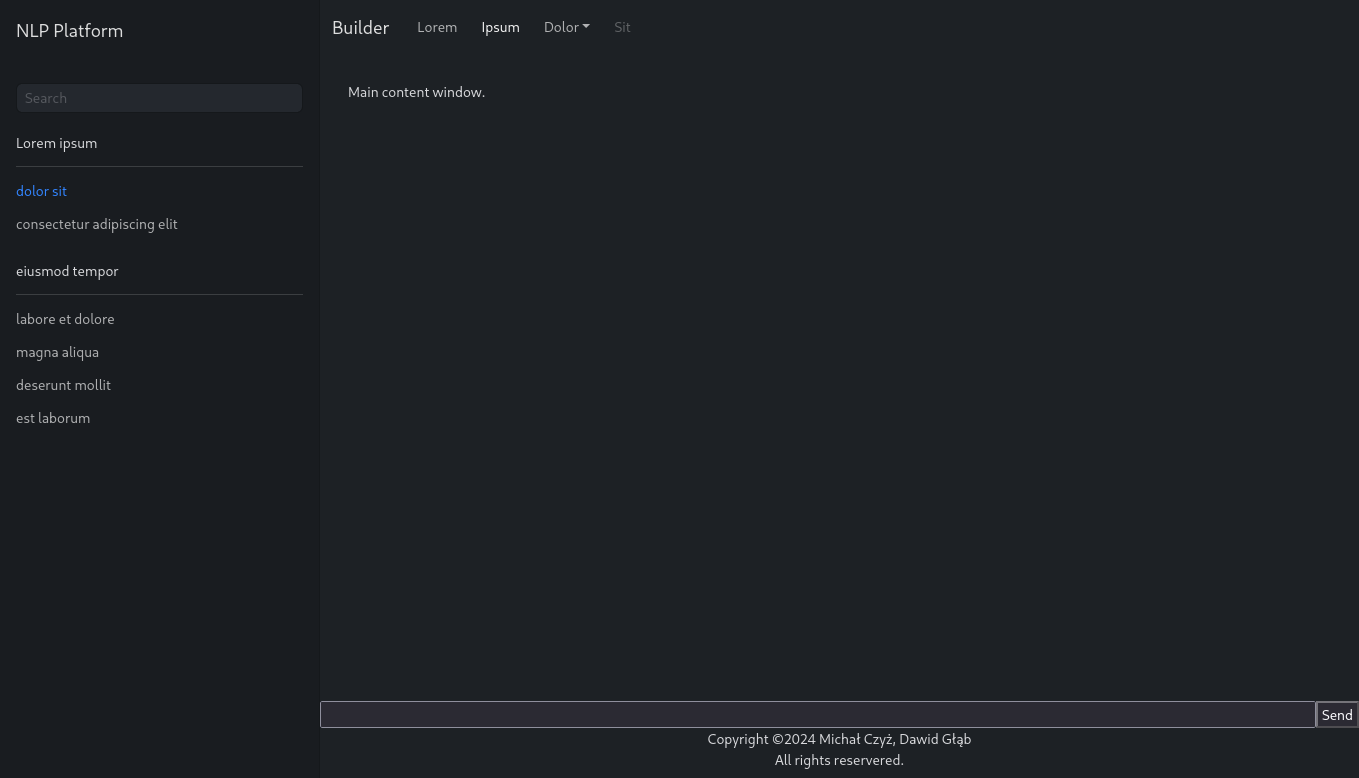
\includegraphics[width=1\linewidth]{ui_mockup.png}
  \caption{\label{fig:ui mockup}Propozycja interfejsu użytkownika.}
\end{figure}

Serwer python oraz program do analizy sentymentu nie będzie zawierał ui. Jedyna komunikacja z tymi warstwami będzie możliwa poprzez API(JS<->Python) lub RPC (Python<->C++)

\section{Diagram klas}

\begin{figure}
\centering
    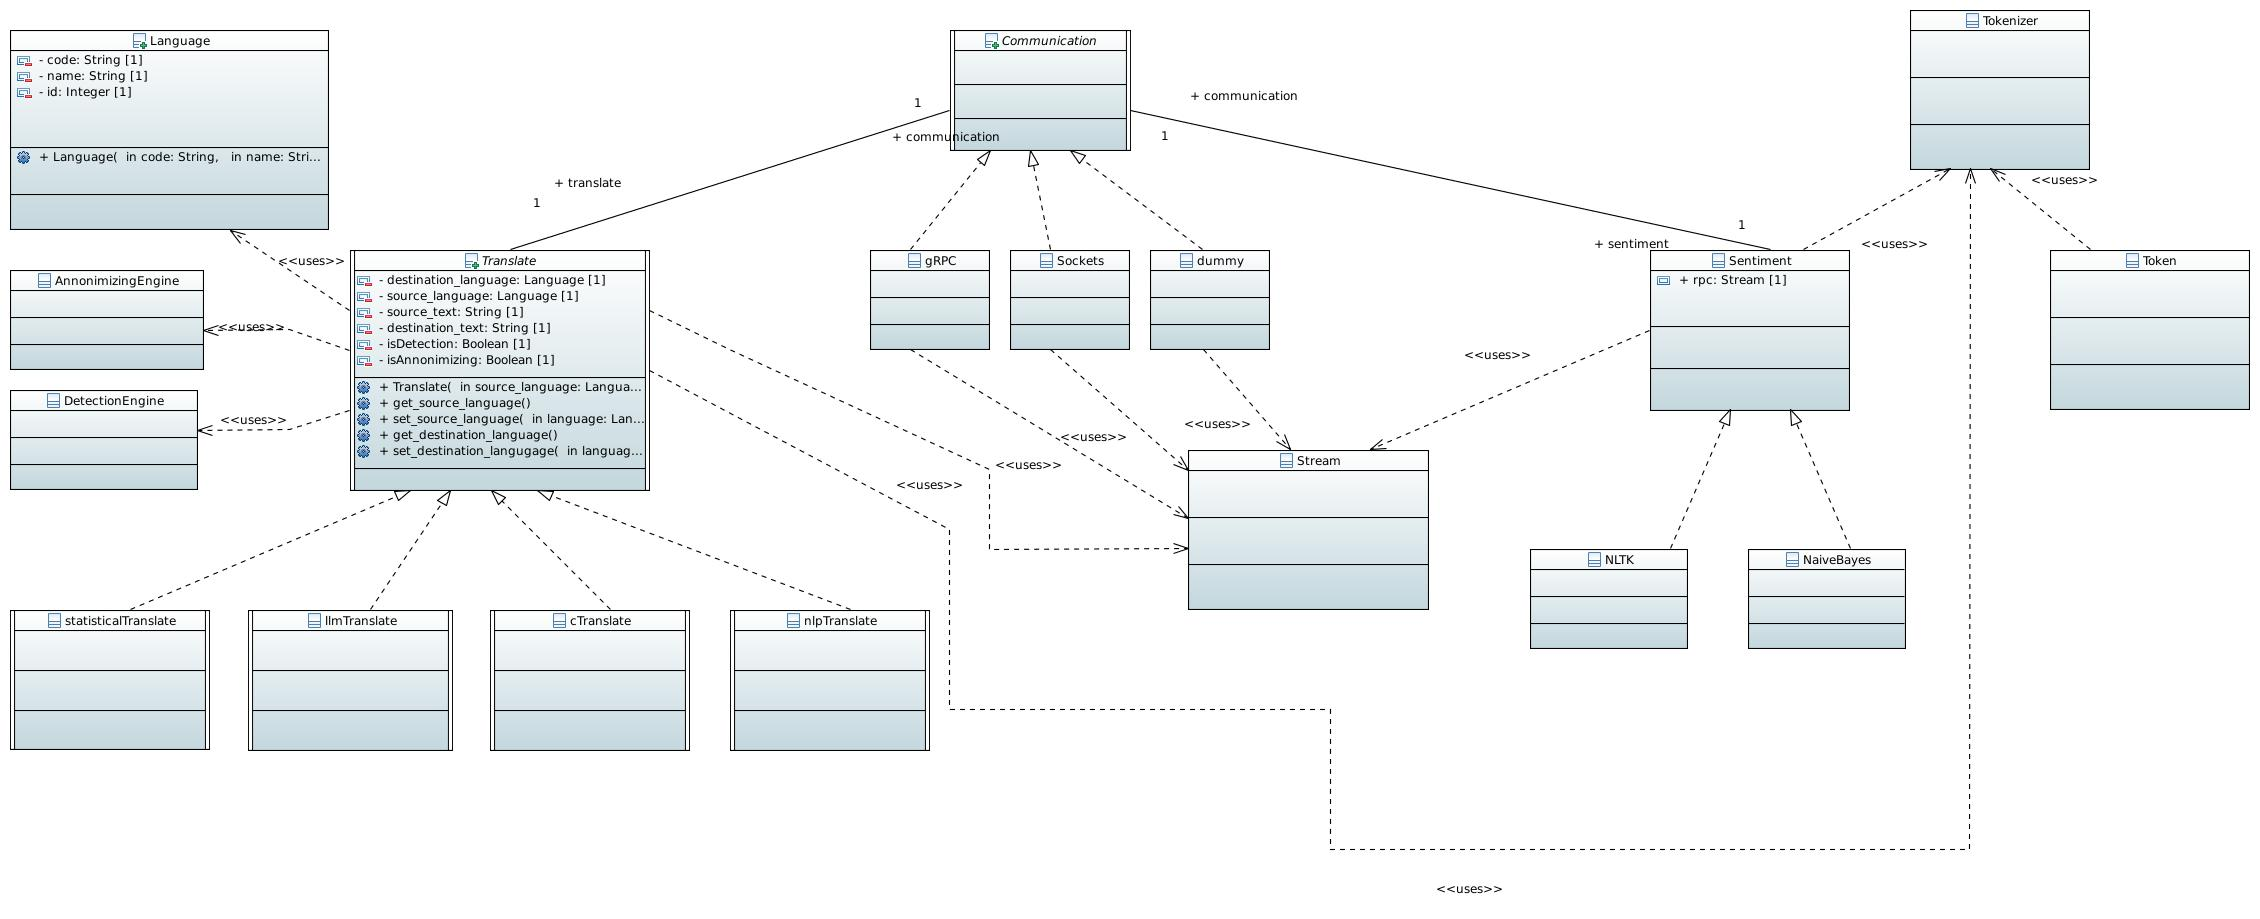
\includegraphics[width=1\linewidth]{Class_Diagram.JPG}
    \caption{\label{fig:Class Diagram}Proponowany diagram klas.}
\end{figure}

Główną abstrakcją części wykrywającej sentyment będzie klasa Sentiment która będzie dziedziczyć poszczególne tryby analizy jako klasy i wysyłać wynik działania poprzez klasę Stream zawierającą połączenie RPC.

\end{document}
